\documentclass[authoryearcitations]{UoYCSproject}

\usepackage[margin=2cm]{geometry}
\usepackage[matrix,frame,arrow]{xypic}
\usepackage{graphicx}
\usepackage{qtree}
%    Q-circuit version 1.2
%    Copyright (C) 2004  Steve Flammia & Bryan Eastin, 4/23/06
%    This program is free software; you can redistribute it and/or modify
%    it under the terms of the GNU General Public License as published by
%    the Free Software Foundation; either version 2 of the License, or
%    (at your option) any later version.
%
%    This program is distributed in the hope that it will be useful,
%    but WITHOUT ANY WARRANTY; without even the implied warranty of
%    MERCHANTABILITY or FITNESS FOR A PARTICULAR PURPOSE.  See the
%    GNU General Public License for more details.
%
%    You should have received a copy of the GNU General Public License
%    along with this program; if not, write to the Free Software
%    Foundation, Inc., 59 Temple Place, Suite 330, Boston, MA  02111-1307  USA

\usepackage[matrix,frame,arrow]{xy}
\usepackage{amsmath}
\newcommand{\bra}[1]{\left\langle{#1}\right\vert}
\newcommand{\ket}[1]{\left\vert{#1}\right\rangle}
    % Defines Dirac notation.
\newcommand{\qw}[1][-1]{\ar @{-} [0,#1]}
    % Defines a wire that connects horizontally.  By default it connects to the object on the left of the current object.
    % WARNING: Wire commands must appear after the gate in any given entry.
\newcommand{\qwx}[1][-1]{\ar @{-} [#1,0]}
    % Defines a wire that connects vertically.  By default it connects to the object above the current object.
    % WARNING: Wire commands must appear after the gate in any given entry.
\newcommand{\cw}[1][-1]{\ar @{=} [0,#1]}
    % Defines a classical wire that connects horizontally.  By default it connects to the object on the left of the current object.
    % WARNING: Wire commands must appear after the gate in any given entry.
\newcommand{\cwx}[1][-1]{\ar @{=} [#1,0]}
    % Defines a classical wire that connects vertically.  By default it connects to the object above the current object.
    % WARNING: Wire commands must appear after the gate in any given entry.
\newcommand{\gate}[1]{*{\xy *+<.6em>{#1};p\save+LU;+RU **\dir{-}\restore\save+RU;+RD **\dir{-}\restore\save+RD;+LD **\dir{-}\restore\POS+LD;+LU **\dir{-}\endxy} \qw}
    % Boxes the argument, making a gate.
\newcommand{\meter}{\gate{\xy *!<0em,1.1em>h\cir<1.1em>{ur_dr},!U-<0em,.4em>;p+<.5em,.9em> **h\dir{-} \POS <-.6em,.4em> *{},<.6em,-.4em> *{} \endxy}}
    % Inserts a measurement meter.
\newcommand{\measure}[1]{*+[F-:<.9em>]{#1} \qw}
    % Inserts a measurement bubble with user defined text.
\newcommand{\measuretab}[1]{*{\xy *+<.6em>{#1};p\save+LU;+RU **\dir{-}\restore\save+RU;+RD **\dir{-}\restore\save+RD;+LD **\dir{-}\restore\save+LD;+LC-<.5em,0em> **\dir{-} \restore\POS+LU;+LC-<.5em,0em> **\dir{-} \endxy} \qw}
    % Inserts a measurement tab with user defined text.
\newcommand{\measureD}[1]{*{\xy*+=+<.5em>{\vphantom{\rule{0em}{.1em}#1}}*\cir{r_l};p\save*!R{#1} \restore\save+UC;+UC-<.5em,0em>*!R{\hphantom{#1}}+L **\dir{-} \restore\save+DC;+DC-<.5em,0em>*!R{\hphantom{#1}}+L **\dir{-} \restore\POS+UC-<.5em,0em>*!R{\hphantom{#1}}+L;+DC-<.5em,0em>*!R{\hphantom{#1}}+L **\dir{-} \endxy} \qw}
    % Inserts a D-shaped measurement gate with user defined text.
\newcommand{\multimeasure}[2]{*+<1em,.9em>{\hphantom{#2}} \qw \POS[0,0].[#1,0];p !C *{#2},p \drop\frm<.9em>{-}}
    % Draws a multiple qubit measurement bubble starting at the current position and spanning #1 additional gates below.
    % #2 gives the label for the gate.
    % You must use an argument of the same width as #2 in \ghost for the wires to connect properly on the lower lines.
\newcommand{\multimeasureD}[2]{*+<1em,.9em>{\hphantom{#2}}\save[0,0].[#1,0];p\save !C *{#2},p+LU+<0em,0em>;+RU+<-.8em,0em> **\dir{-}\restore\save +LD;+LU **\dir{-}\restore\save +LD;+RD-<.8em,0em> **\dir{-} \restore\save +RD+<0em,.8em>;+RU-<0em,.8em> **\dir{-} \restore \POS !UR*!UR{\cir<.9em>{r_d}};!DR*!DR{\cir<.9em>{d_l}}\restore \qw}
    % Draws a multiple qubit D-shaped measurement gate starting at the current position and spanning #1 additional gates below.
    % #2 gives the label for the gate.
    % You must use an argument of the same width as #2 in \ghost for the wires to connect properly on the lower lines.
\newcommand{\control}{*!<0em,.025em>-=-{\bullet}}
    % Inserts an unconnected control.
\newcommand{\controlo}{*-<.21em,.21em>{\xy *=<.59em>!<0em,-.02em>[o][F]{}\POS!C\endxy}}
    % Inserts a unconnected control-on-0.
\newcommand{\ctrl}[1]{\control \qwx[#1] \qw}
    % Inserts a control and connects it to the object #1 wires below.
\newcommand{\ctrlo}[1]{\controlo \qwx[#1] \qw}
    % Inserts a control-on-0 and connects it to the object #1 wires below.
\newcommand{\targ}{*!<0em,.019em>=<.79em,.68em>{\xy {<0em,0em>*{} \ar @{ - } +<.4em,0em> \ar @{ - } -<.4em,0em> \ar @{ - } +<0em,.36em> \ar @{ - } -<0em,.36em>},<0em,-.019em>*+<.8em>\frm{o}\endxy} \qw}
    % Inserts a CNOT target.
\newcommand{\qswap}{*=<0em>{\times} \qw}
    % Inserts half a swap gate. 
    % Must be connected to the other swap with \qwx.
\newcommand{\multigate}[2]{*+<1em,.9em>{\hphantom{#2}} \qw \POS[0,0].[#1,0];p !C *{#2},p \save+LU;+RU **\dir{-}\restore\save+RU;+RD **\dir{-}\restore\save+RD;+LD **\dir{-}\restore\save+LD;+LU **\dir{-}\restore}
    % Draws a multiple qubit gate starting at the current position and spanning #1 additional gates below.
    % #2 gives the label for the gate.
    % You must use an argument of the same width as #2 in \ghost for the wires to connect properly on the lower lines.
\newcommand{\ghost}[1]{*+<1em,.9em>{\hphantom{#1}} \qw}
    % Leaves space for \multigate on wires other than the one on which \multigate appears.  Without this command wires will cross your gate.
    % #1 should match the second argument in the corresponding \multigate. 
\newcommand{\push}[1]{*{#1}}
    % Inserts #1, overriding the default that causes entries to have zero size.  This command takes the place of a gate.
    % Like a gate, it must precede any wire commands.
    % \push is useful for forcing columns apart.
    % NOTE: It might be useful to know that a gate is about 1.3 times the height of its contents.  I.e. \gate{M} is 1.3em tall.
    % WARNING: \push must appear before any wire commands and may not appear in an entry with a gate or label.
\newcommand{\gategroup}[6]{\POS"#1,#2"."#3,#2"."#1,#4"."#3,#4"!C*+<#5>\frm{#6}}
    % Constructs a box or bracket enclosing the square block spanning rows #1-#3 and columns=#2-#4.
    % The block is given a margin #5/2, so #5 should be a valid length.
    % #6 can take the following arguments -- or . or _\} or ^\} or \{ or \} or _) or ^) or ( or ) where the first two options yield dashed and
    % dotted boxes respectively, and the last eight options yield bottom, top, left, and right braces of the curly or normal variety.
    % \gategroup can appear at the end of any gate entry, but it's good form to pick one of the corner gates.
    % BUG: \gategroup uses the four corner gates to determine the size of the bounding box.  Other gates may stick out of that box.  See \prop. 
\newcommand{\rstick}[1]{*!L!<-.5em,0em>=<0em>{#1}}
    % Centers the left side of #1 in the cell.  Intended for lining up wire labels.  Note that non-gates have default size zero.
\newcommand{\lstick}[1]{*!R!<.5em,0em>=<0em>{#1}}
    % Centers the right side of #1 in the cell.  Intended for lining up wire labels.  Note that non-gates have default size zero.
\newcommand{\ustick}[1]{*!D!<0em,-.5em>=<0em>{#1}}
    % Centers the bottom of #1 in the cell.  Intended for lining up wire labels.  Note that non-gates have default size zero.
\newcommand{\dstick}[1]{*!U!<0em,.5em>=<0em>{#1}}
    % Centers the top of #1 in the cell.  Intended for lining up wire labels.  Note that non-gates have default size zero.
\newcommand{\Qcircuit}[1][0em]{\xymatrix @*[o] @*=<#1>}
    % Defines \Qcircuit as an \xymatrix with entries of default size 0em.  The optional argument, #1, is for use with clusters, and allows you
    % to fix the size of the nodes.  I would not advise using it with normal circuits.
\newcommand{\node}[2][]{{\begin{array}{c} \ _{#1}\  \\ {#2} \\ \ \end{array}}\drop\frm{o} }
    % When Qcircuit has been passed the optional argument for cluster states, this command produces a round node of the size specified in that
    % argument.  The optional argument #2 specifies the contents of a node, while optional argument #1 is a secondary label.  
\newcommand{\link}[2]{\ar @{-} [#1,#2]}
    % Draws a wire or connecting line to the element #1 rows down and #2 columns forward.
\newcommand{\pureghost}[1]{*+<1em,.9em>{\hphantom{#1}}}
    % Same as \ghost except it omits the wire leading to the left. 

\vfuzz2pt % Don't report over-full v-boxes if over-edge is small

\author{Sam Ratcliff}
\title{Quantum Algorithm Synthesis Workbench}
\date{\today}
\supervisor{John A Clark}
\MEng
\wordcount{8832}
\setcounter{tocdepth}{3}
\includes{}

\excludes{}

\abstract{ TO BE DONE
}

\begin{document}
\maketitle
%PUT THESE BACK IN
\listoffigures
\listoftables
% \renewcommand*{\lstlistlistingname}{List of Listings}
% \lstlistoflistings

\chapter{Introduction}
\chapter{Literature Review}
\section{Introduction to Quantum Computation}
%Historic Introduction
In 1980, Richard Feynman noted `it is impossible to represent the results of quantum mechanics with a classical universal device`\cite{Feynman82simulatingphysics}.
This statement was a seed for interest in the field of Quantum Computation.
The true power of quantum computation was not initially realised.
The discovery of a quantum algorithm by David Deutsch\cite{Deutsch1985} in 1985 that performed better than a classical computer was the first glimpse of the potential power provided by harnessing quantum mechanics.
However, with slow progress of research into both their implementation and algorithms, the energy behind the research started to decrease.
It would take a discovery by Peter Shor\cite{Shor:1994jg} to reignite the excitement surrounding the subject.  

%What is Quantum Computation
In classical computers the computation is performed using the discrete values of $0$ and $1$.
These values are indicated by +$5$V and $0$V signals propagating round circuits.
A signal can only be $0$ or $1$, there is no in between value.
Each signal can indicate the value of a single 'bit' of data.
A combination of n bits can be used to represent a number from $0$ to $2^n-1$, an n-bit number.
Classical computation works through the manipulation of these n-bit numbers.


Quantum Computation uses the properties of quantum mechanics to perform computation.
The power of quantum computers come from the use of particles in superpositions.
% This can be seen as the particle being both a $0$ and $1$ simultaneously.
Qubits are the quantum equivalent of the classical bit.
It is these qubits which can be placed into superpositions.
Just as classical computers manipulate bits to perform computation, quantum computers manipulate qubits and their superpositions to perform computation.
The power of these superpositions is not obviously apparent.

It is not possible to observe the superposition of a particle.
When observed the superposition 'collapses' to either logical $0$ or $1$, the basis states.
The probability the the superposition collapses to $0$ is determined by the superposition's properties.

%Explanation of Bra-Ket notation
To write the state of a superposition it is usual to use the 'Bra-Ket' notation, introduced by Dirac\cite{dirac2004principles}.
A 'Ket' is mathematical notation, $\vert$a$\rangle$, which represents a basis function of the respective Hilbert space, $\mathcal{H}$, as a column vector.
\begin{equation}
\vert
a
\rangle = 
\begin{pmatrix}
a_1\\
a_2\\
a_3\\
\vdots
\end{pmatrix}
\end{equation}
Hilbert spaces extend the simple Euclidean vector space into a potential infinite dimension function space.
\begin{figure}
\centering
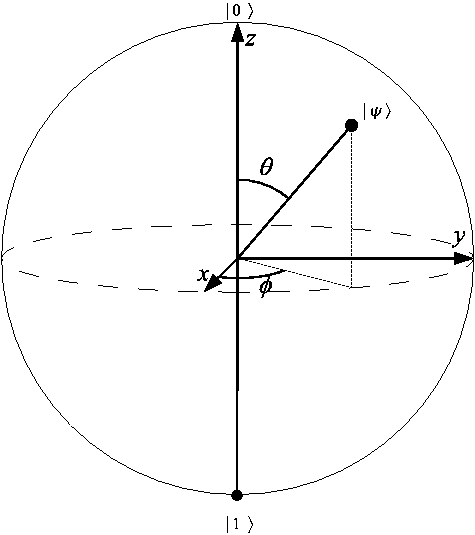
\includegraphics[scale=0.5]{Bloch.png}
\caption{The 1-Qubit Bloch Sphere \cite{QuantikiBlochSphereImage}}
\label{BlochSphere}
\end{figure}
A quantum state space can also been visualised in terms of the Bloch sphere, shown in Figure \ref{BlochSphere}.
The shown Bloch sphere is for a single qubit system, it can be extended to an n-qubit system however the visualisation breaks down.
All 'pure' quantum states can be described using the Bloch sphere and all exist on the surface produced by the unit sphere.
In this report only pure quantum states will be used and all explanation of quantum states are more precisely explanations of 'pure' quantum states.
This means that all superpositions of states can be expressed in terms of $|\psi\rangle = \cos \frac{\theta}{2} \, |0 \rangle +  e^{i \phi}  \sin \frac{\theta}{2}  \,|1 \rangle $ with $0 \leq \theta \leq \pi, \quad  0 \leq \phi \leq 2 \pi$, ignoring global phase factors\cite{BlochSphereTalk}.

In quantum mechanics, Kets are used to indicate a state, for example $\vert$0$\rangle$ is the state of a logical $0$ whereas $\vert$1$\rangle$ is the state of logical $1$.
Using this notation and the inclusion of probabilities, the state of the superposition can be expressed.

A dual to the Ket notation is the 'Bra' notation, $\langle$a$\vert$.
This notation is used to denote the 'dual vector' of the corresponding Ket.
For a state vector represented by
\begin{equation}\label{ket_explanation_example}
\vert
a
\rangle = 
\begin{pmatrix}
a_1\\
a_2\\
a_3\\
\vdots
\end{pmatrix}
\end{equation}
there is a dual vector representing its Hermitian conjugate
\begin{equation}\label{bra_explanation_example}
\langle
a
\vert = 
\begin{pmatrix}
a_1^*$$
a_2^*$$
a_3^*$$
\cdots
\end{pmatrix}
\end{equation}

Combining the two vectors $\langle$a$\vert$ and $\vert$b$\rangle$, written $\langle$a$\vert\vert$b$\rangle$, represents the inner product of the two vectors.
If a and b are unit vectors and $a == b$, $\langle$a$\vert\vert$b$\rangle == 1$.
If a and b are orthogonal, $\langle$a$\vert\vert$b$\rangle == 0$.

The outer product of two vectors, a and b, can be represented by $\vert$a$\rangle$$\langle$b$\vert$.
This represents the transformation from a to b.
It can also be represented in matrix form.

With
$\vert
0
\rangle
== 
\begin {pmatrix}
1\\
0\\
\end{pmatrix}
$
and
$\vert
1
\rangle
==  
\begin {pmatrix}
0\\
1\\
\end{pmatrix}
$
it is possible to represent $1$-qubit operations in the bra-ket notation.
For example, the NOT gate performs a simple negation of a qubit's value.
This can be written as $\vert0\rangle\langle1\vert + \vert1\rangle\langle0\vert$.
Substituting in the vector values we have
\begin{equation}
\begin{tabular}{ r c l }
\(\begin {pmatrix}
1\\
0
\end{pmatrix}
\begin {pmatrix}
0&&
1
\end{pmatrix}
 + 
\begin {pmatrix}
0\\
1
\end{pmatrix}
\begin {pmatrix}
1&&
0
\end{pmatrix}\)
& \(=\)
& \( 
\begin{pmatrix}
0 && 1 \\
0 && 0
\end{pmatrix}
 + 
\begin{pmatrix}
0 && 0\\
1 && 0
\end{pmatrix}
\) \\
& \(=\)
& \( 
\begin{pmatrix}
0 && 1 \\
1 && 0
\end{pmatrix}
\)
\end{tabular}
\end{equation}

This matrix can be seen as a transformation matrix for the NOT operation.
In quantum computation, the NOT gate is one of the $4$ gates known as the Pauli gates, more specifically the Pauli-X gate.
It is called the Pauli-X gate as it can be seen as a rotation of $\pi$ radians about the X axis of the Bloch sphere, Figure \ref{BlochSphere}.

% Definition of Unitary
The matrices representing the Pauli-X gate and all other quantum logic gates are unitary.
A unitary matrix, U, is one which adheres to
\begin{equation}
U*{\dagger}
U == UU*{\dagger} = I_N
\end{equation}
where $I_N$ is the identity matrix in N dimensions and $U*{\dagger}$ is the complex conjugate of $U$.
% Reversible logic
The implication of all quantum logic operations being unitary is that they are reversible, this is a difference to classical computation.
With many classical logic gates irreversible, there is not a set of quantum logic gates which is as computationally powerful as the set of classical logic gates.
This seems like a major issue, quite the contrary.
The set of classical logic gates can be replaced by reversible equivalents and therefore it is possible to produce a set of quantum logic gates with the equivalent computational power as the classical logic gates.

%Superposition
As with all probabilities, the overall probability of a superposition collapsing to any of the states it contains must equal $1$.
\begin{equation}
\label{superposition_explanaiton}
\alpha\vert0\rangle+\beta\vert1\rangle
\end{equation}
\begin{equation}
\label{superposition_explanaiton_sum}
\frac{1}{2^{\frac{1}{n}}}\sum\limits_{i=0}^N \ket{x_i}
\end{equation}
Equation \eqref{superposition_explanaiton} is how the combination of the logical $0$ and $1$ states in a superposition can be represented for a single particle.
It can also be represented in the for of Equation \eqref{superposition_explanaiton}.
This is equivalent to the representation provided by the Bloch sphere, Figure \ref{BlochSphere}.
The probability of this state collapsing to the basis state $0$ can be calculated by $\vert\alpha\vert^2$ where $\alpha$ is a complex number.
$\alpha$ is known as the probability amplitude of $\vert0\rangle$.
Similarly, the probability of this state collapsing to the basis state $1$ can be calculated by $\vert\beta\vert^2$, $\beta$ being the probability amplitude of $\vert1\rangle$.
It follows that $\frac{1}{\sqrt{2}}\vert0\rangle+\frac{1}{\sqrt{2}}\vert1\rangle$ is an equal superposition where the collapse to 0 is just as likely as collapsing to $1$.
This provides the first glimpse of where a single qubit has the ability to perform a function not currently possible on a classical computer.
With n-qubits in the equal superposition, we have n binary values which have an equal probability of taking the value $0$ as the value $1$.
With an ordering decided of these qubits, collapsing the superposition of each qubit will result in a binary value of length n.
With all probabilities being $\frac{1}{2}$ this binary value takes a truly random value between $0$ and $2^n-1$.
It is not possible to produce a truly random number using a classical computer.

A second indication of the power held within the idea of superposition becomes clear if we look at the n-qubits in their equal superposition.
In 1935, Erwin Schr$\ddot{o}$ginger\cite{SchroedingersCat} proposed a thought experiment to explain the idea of superposition.
Imagine a cat in a fully opaque box with a vile of poison.
The vile may break at any time, a truly random variable.
After sealing the box the state of the cat is not known.
The cat could be alive if the vile has not broken but could just as likely be dead.
Only by looking inside the box will the state of the cat be known.
Until this time the cat could be thought of as both alive and dead at the same time.
If we assign 'dead' to the state $\vert0\rangle$ and 'alive' to the state $\vert1\rangle$ the situation looks very similar to the state we have previously seen.
Therefore, just as the cat can be thought of as both dead and alive at the same time, a qubit in the superposition $\frac{1}{\sqrt{2}}\vert0\rangle+\frac{1}{\sqrt{2}}\vert1\rangle$ can be thought of as both 0 and 1 at the same time.
This leads to a very powerful property of quantum computers.
With n classical bits, a single number in the range 0 to $2^n-1$ can be expressed at any one time.
With n quantum qubits, every number in the range 0 to $2^n-1$ can be expressed at any one time.
This effectively allows computation over the whole range of $2^n$ inputs to be carried out in parallel.

This parallelism is very powerful and has been shown to enable the computation of problems classified as NP to be performed in polynomial time.
This does however have a caveat.
As mentioned previously the superposition cannot itself be observed or measured.
When observed the superposition collapses to a basis state with respect to the superposition probability amplitudes.
This means that even though $2^n$ calculations can be performed in parallel, only a single answer can be observed.

% mathematic examples of matrices and the application
Along with the Pauli-X gate, there are an additional 3 Pauli gates.
The Pauli-I gate is the simplest of all quantum gates.
It is the identity gate, the output is identical to the input.
In Dirac notation this is $\vert0\rangle\langle0\vert + \vert1\rangle\langle1\vert$, and in matrix form below
\begin{equation}
\begin{tabular}{ r c l }
\(\begin {pmatrix}
1\\
0
\end{pmatrix}
\begin {pmatrix}
1&&
0
\end{pmatrix}
 + 
\begin {pmatrix}
0\\
1
\end{pmatrix}
\begin {pmatrix}
0&&
1
\end{pmatrix}\)
& \(=\)
& \( 
\begin{pmatrix}
1 && 0 \\
0 && 0
\end{pmatrix}
 + 
\begin{pmatrix}
0 && 0\\
0 && 1
\end{pmatrix}
\) \\
& \(=\)
& \( 
\begin{pmatrix}
1 && 0 \\
0 && 1
\end{pmatrix}
\)
\end{tabular}
\end{equation}

The Pauli-Z gate is similar to the Pauli-X gate, but differs in the axis about which it performs the rotation.
The Pauli-Z gate rotates the quantum state by $\pi$ radians about the Z axis.
This represents a phase flip of the quantum state.
The phase of a state is important when interference is used in computation.
In Dirac notation this is $\vert0\rangle
\langle0\vert + \vert1\rangle(-\langle1\vert$), and in matrix form below
\begin{equation}
\begin{tabular}{ r c l }
\(\begin {pmatrix}
1\\
0
\end{pmatrix}
\begin {pmatrix}
1&&
0
\end{pmatrix}
 + 
\begin {pmatrix}
0\\
1
\end{pmatrix}
\begin {pmatrix}
0&&
-1
\end{pmatrix}\)
& \(=\)
& \( 
\begin{pmatrix}
1 && 0 \\
0 && 0
\end{pmatrix}
 + 
\begin{pmatrix}
0 && 0\\
0 && -1
\end{pmatrix}
\) \\
& \(=\)
& \( 
\begin{pmatrix}
1 && 0 \\
0 && -1
\end{pmatrix}
\)
\end{tabular}
\end{equation}

The Pauli-Y gate is similar to both the Pauli-X and Pauli-Z gates, but differs in the axis about which it performs the rotation.
The Pauli-Y gate rotates the quantum state by $\pi$ radians about the Y axis.
This represents a phase flip followed by a bit flip.
In Dirac notation this is $\vert0\rangle
(i\langle1\vert) + \vert1\rangle(-i\langle0\vert$), and in matrix form below
\begin{equation}
\begin{tabular}{ r c l }
\(\begin {pmatrix}
1 \\
0
\end{pmatrix}
\begin {pmatrix}
0 &&
-i
\end{pmatrix}
 + 
\begin {pmatrix}
0 \\
1
\end{pmatrix}
\begin {pmatrix}
i &&
0
\end{pmatrix}\)
& \(=\)
& \( 
\begin{pmatrix}
0 && -i \\
0 && 0
\end{pmatrix}
 + 
\begin{pmatrix}
0 && 0\\
i && 0
\end{pmatrix}
\) \\
& \(=\)
& \( 
\begin{pmatrix}
0 && -i \\
i && 0
\end{pmatrix}
\)
\end{tabular}
\end{equation}

Along with the single qubit operations, like those above, there are operations which can act over n-qubits.
A simple example of a 2 qubit operation is the controlled-NOT, CNOT, operator.
This is a simple extension of the Pauli-X gate.
\begin{table}
\centering
\begin{tabular}{ l | c || r | }
0 & 0 & 0 \\
0 & 1 & 1 \\
1 & 0 & 1 \\
1 & 1 & 0 \\ \end{tabular}
\caption{Classical CNOT Truth Table}
\label{CNOTTruthTable}
\end{table}
The CNOT gate has a control input which it requires to be in the logical $1$ state for the NOT operation on the second input to be carried out.
In classical logic this would extend the truth table to be as shown in Table \ref{CNOTTruthTable}.
The truth table of the CNOT gate is the same as that of the XOR gate.
The Dirac notation of the CNOT gate is $\vert00\rangle\langle00\vert + \vert01\rangle\langle01\vert + \vert10\rangle\langle11\vert + \vert11\rangle\langle10\vert$.

\section{An Introduction to Quantum Algorithms}
%Known Quantum Algorithms

Just as with classical computers, the computation to produce the required output given inputs is given in the form of an algorithm.
Quantum algorithms can be constructed in several ways. These definitions are based on those provided by Massey\cite{masseythesis}.

\begin{itemize}
\item A quantum circuit can be used to represent an algorithm at the level of quantum logic gates.
This is similar to a specific purpose circuit diagram for classical systems.
\item A quantum program is a representation of the algorithm in some higher level quantum 'programming' language which would generate the required circuit.
The circuit generated is not defined in this method, just it's behaviour.
This could be seen as slightly more flexible that the quantum circuit model as the 'compiler' can be updated to reflect the findings of future research.
\item A parameterisable quantum algorithm is a representation in pure Pseudo-code.
It proves the flexibility of changing some value n, which is used to indicate the number of input qubits, to produce quantum circuits or programs with the desired behaviour on n qubits.
This is the most flexible construction of quantum algorithms.
It can cope with the changing in input size and can use findings of research just like in the 'compilation' of a quantum program.
\end{itemize}

Currently there are very few quantum algorithms known.
Peter Shor has carried out, and published, a discussion on the progress made `in discovering algorithms for computation on a quantum computer`\cite{Shor:2004:PQA:1032132.1032149}.
Shor suggests two possible reasons for the lack of quantum algorithms.
The first is `that there might really be only a few problems for which quantum computers can offer a substantial speed-up over classical computers`\cite{Shor:2004:PQA:1032132.1032149}.
This would indeed make the discovery of useful quantum algorithms difficult.
However, I feel this is somewhat pessimistic.
The main focus of the paper published by Feynman\cite{Feynman82simulatingphysics} was the problem of simulating the physics of quantum mechanics on a classical computer.
This to suggests there would be the potential of many applications of quantum computers, even if they aren't analogous to the classical computational applications.

The second is `that quantum computers operate in a manner so non-intuitive, and so different from classical computers`\cite{Shor:2004:PQA:1032132.1032149} that our current algorithm knowledge is close to useless.
This, in my opinion, is a much more believable obstacle.
Quantum mechanics is seen by many as a confusing and mystical subject.
Even prize winning mathematician and physicist Roger Penrose is attributed to the remark `Quantum mechanics makes absolutely no sense`.
Statements like this and the atmosphere surrounding quantum mechanics makes the potential of its study more than some what daunting.
As computer scientists, the exposure to and therefore our understanding of quantum mechanics is limited, in general.
With this in mind it is, currently, unreasonable to expect the discovery of algorithms that exploit the finer details of this complex and subtle theory to become an everyday occurrence.

The following few sections outline a selection of the currently known quantum algorithms.

\subsection{Deutsch-Jozsa Algorithm}
%Deutsch-Jozsa Algorithm
The Deutsch-Jozsa algorithm\cite{1992-deutsch} is a generalisation and improvement over an earlier algorithm proposed by David Deutsch\cite{Deutsch1985}.
The algorithm described here will be the algorithm including the improvements published in \cite{Macchiavello97quantumalgorithms}, the resulting algorithm is still refereed to as the Deutsch-Jozsa algorithm.

The original Deutsch algorithm\cite{Deutsch1985} was proposed to solve the following problem:
\begin{quote}
Given a function f:{0,1}$\to${0,1}, decide whether it is either a balanced, or constant function.
The function f is guaranteed to be either constant or balanced.
\end{quote}
The algorithm proposed was not deterministic, but provided the correct answer with probability $\frac{1}{2}$.
The algorithm's major breakthrough was that it only required a single invocation of the function f to decide on which category it belonged.
This is compared to the best classical approach requiring two invocations to the function.
This was the first algorithm that it was possible to compute the solution to a problem more efficiently than a classical computer by exploiting quantum mechanics.
The uncertainty of the result was obviously a problem but the principle was a large break through.

In 1992, David Deutsch and Richard Jozsa\cite{1992-deutsch} presented an improvement and extension which allowed for functions $f:{0,1}^{2n}\to{0,1}$ to be categorised as constant of balanced.
The algorithm was again probabilistic but also required 2 invocations to the function f.
This means that in the worst case, with $f_1:{0,1}\to{0,1}$, the algorithm will perform worst than both the original Deutsch algorithm\cite{Deutsch1985} and the classical algorithm due to the probabilistic nature of its result.
This is a very limited case and does improve as the value of n increases.
As with the original algorithm, the number of invocations of f is constant, truly independent of both n and f.
This again is an improvement over the classical algorithm which requires in the worst case $2^n+1$ to be certain of the function's category.
\begin{figure}
\[
\Qcircuit @C=1.0em @R=.7em {
& \lstick{\ket{0}} & \gate{H} & \multigate{3}{\mathcal{F}} & \gate{H} & \qw \\
& \lstick{\ket{0}} & \gate{H} & \ghost{\mathcal{F}} & \gate{H} & \qw \\
& \lstick{\ket{0}} & \gate{H} & \ghost{\mathcal{F}} & \gate{H} & \qw \\
& \lstick{\ket{0}} & \gate{H} & \ghost{\mathcal{F}}  & \gate{H} & \qw \\
& \lstick{\ket{1}} & \gate{H} & \targ\qwx & \qw &  \rstick{\ket{0}-\ket{1}}\qw 
}
\]
\caption{Deutsch-Jozsa Circuit}
 \label{Deutsch-Jozsa-Cir}
\end{figure}

The algorithm requires n input qubits and a single control qubit.
The n input qubits are initialised to $\ket{0}$.
The control qubit is initialised to $\ket{1}$.
The n-fold Hadamard gates are then used to produce the superposition of all $2^n-1$ possible inputs, $x = (\ket{0}+\ket{1})^n)$.
The Hadamard gate on the control qubit is used to produce the superposition $\ket{0}-\ket{1}$.
The difference in superpositions between the input and control qubits is important to the way in which the algorithm classifies a function.
This produces a state  $(\ket{0}+\ket{1})^n(\ket{0}-\ket{1})$.

The n input qubits are then passed to the function we was to classify, f.
The result of f for the x input is used as the control for a CNOT gate acting on the control qubit.
Remember at this point that the input x is in effect all possible inputs to f, and as such the output is all the respective outputs.
This means that each of the factors of the input are transformed, based on the action of f.
This can be formalised as $U_f(\ket{x},\ket{y})=(\ket{x},\ket{f(x)\otimes{y}})$.
Using the final Hadamard gates we can use the transformation to categorise f.

If we assume n to be equal to 4, then after the initial Hadamard gates we have the superposition:
\begin{equation}
\frac{1}{2}\ket{\Psi_{init}}\frac{1}{\sqrt{2}}(\ket{0}-\ket{1})=\frac{1}{2}(\ket{00}+\ket{01}+\ket{10}+\ket{11})\frac{1}{\sqrt{2}}(\ket{0}-\ket{1})
\end{equation}
At this point it is worth mentioning an identity which will be used in this explanations.
\begin{equation}
(\ket{b}-\ket{a})\equiv-1(\ket{a}-\ket{b})
\end{equation}
and by linearity
\begin{equation}
\ket{a}(\ket{c}-\ket{b})\equiv\ket{a}(-1(\ket{b}-\ket{c}))\equiv-1\ket{a}(\ket{b}-\ket{c})
\label{target_qubit_identity}
\end{equation}
The CNOT on the target qubit is only activated if $f(x)=1$ which, using the equivalent above, produces the superposition $-1(\ket{0}-\ket{1})$.
This can also be generalised as $(-1)^{f(x)}(\ket{0}-\ket{1})$ where $-1^1=-1$ and $-1^0=1$ by definition.
By linearity the superposition after the CNOT controlled by f(x) on the target qubit becomes
\begin{equation}
\frac{1}{2}((-1)^{f(00)}\ket{00}+(-1)^{f(01)}\ket{01}+(-1)^{f(10)}\ket{10}+(-1)^{f(11)}\ket{11})\frac{1}{\sqrt{2}}(\ket{0}-\ket{1})
\end{equation}

After the application of f, the target bit has served it purpose and is neither measured nor entangled with any of the qubits from the n qubit input.
To simplify the equations I will now ignore the $(\frac{1}{\sqrt{2}}\ket{0}-\ket{1})$ contributed by the target qubit, the remaining state will be refereed to as $\Psi$.
If the function f is constant:
\begin{equation}
\ket{\Psi_{const}}=\pm\frac{1}{2}(\ket{00}+\ket{01}+\ket{10}+\ket{11})\frac{1}{\sqrt{2}}(\ket{0}-\ket{1})
\end{equation}
Whereas if f is balanced then:
\begin{equation}
\ket{\Psi_{bal}}=(-1)^{f(00)}\ket{00}+(-1)^{f(01)}\ket{01}+(-1)^{f(10)}\ket{10}+(-1)^{f(11)}\ket{11}
\end{equation}
However,as $\ket{\Psi_{const}}$ and $\ket{\Psi_{bal}}$ are orthogonal we can use this to detect if the function is balanced or constant.
\begin{equation}
\ket{\Psi_{bal}}\bullet\ket{\Psi_{const}} = 0
\end{equation}

Applying the n Hadamard gates to the state $\Psi_{const}$ produces the state $\pm\ket{0}^n$.
When measured this will return the result $0$ as the global phase factor $\pm'$ cannot be observed.
As we have noted, $\Psi_{const}$ is orthogonal to $\Psi_{bal}$ so when the n Hadamard gates are applied the measured result will be anything orthogonal to $0$.
This gives us a clear way of distinguishing between whether f is constant of balanced with certainty and only a single invocation of f.
If the measurement returns $0$ then f is constant, if the measurement returns anything else f is balanced  

% \subsection{Shor's Factorisation Algorithm}
% %Shors Algorithm
% In 1994, Peter Shor astonished the computer science community with a quantum factorisation algorithm.
% This allowed the factorisation of integer numbers into their constituent primes in polynomial time.
% This algorithm is not a pure quantum algorithm, but a hybrid algorithm.
% It has both a quantum and classical portion.



% (READ PAPER) 

\subsection{Grover's Search Algorithm}	
%Grovers Database search algorithm
The Grover Search algorithm\cite{Grover:1996rk} is an unstructured search problem.
The algorithm assumes no underlying structure in the search space.
By this I mean the algorithm does not exploit, and therefore assume, any structure, such as sorting, in the data set being searched.

It has previously been proven\cite{Bennett:1996iu} that the lower complexity limit for any algorithm identifying an element without knowledge of underlying structure in the data is $\Omega(\sqrt{N})$.
For simplicities sake we assume $N=2^n$.
The complexity is measured by the number of elements which need to be queried in order to find the desired element.
The Grover Search algorithm has the complexity $O(\sqrt{N})$ and so `is within a constant factor of the fastest possible quantum mechanical algorithm`\cite{Grover:1996rk}.

\begin{figure}
\[
\Qcircuit @C=1.0em @R=.7em {
& \qw & \qw & \multigate{3}{f} &\qw &  \gate{H} &\qw & \multigate{3}{f_0} &\qw &  \gate{H}  &\qw &\qw\\
& \vdots & &  \ghost{f} & \qw & \vdots & & \ghost{f_0} &\qw &  \vdots & &\qw\\
& \vdots & & \ghost{f} & \qw & \vdots & & \ghost{f_0} &\qw &  \vdots & &\qw\\
& \qw &\qw &  \ghost{f} & \qw & \gate{H} &\qw & \ghost{f_0} &\qw &  \gate{H} &\qw &\qw\\
& \qw &\qw &  \targ \qwx &\qw &  \qw &\qw & \targ \qwx &\qw &  \gate{X} &\qw &\qw 
}
\]
\caption{Grover's Search Circuit}
 \label{Grovers-Search-Cir}
\end{figure}


The mechanisms used within the algorithm to produce a solution to the problem is more subtle than those used but the Deutsch-Jozsa algorithm.
The algorithm does not perform the computation in a single step.
The algorithm requires $O(\sqrt{N})$ steps.
The section of circuit which is repeated is that shown in Figure \ref{Grovers-Search-Cir}.

The algorithm is to initialise the state, $\Psi$, using n Hadamard gates.
\begin{equation}
\Psi_1=\frac{1}{2^{\frac{1}{n}}}\sum\limits_{i=0}^N \ket{x_i}(\ket{0}-\ket{1})
\end{equation}
The application of f is used in an analogous way to in the Deutsch-Jozsa algorithm.
It can again be written as $U_f(\ket{x},\ket{y})=(\ket{x},\ket{f(x)\otimes{y}})$ and remember
\begin{equation}
x_i\epsilon\{x_0,x_1,\ldots,x_{n-1}\}
\end{equation}
\begin{equation}
f(x_i)=1
\end{equation}
\begin{equation}
\forall{x_j} : i\neq{j} : f(x_j)=0
\end{equation}
Just as in the Deutsch-Jozsa algorithm, the result of a $1$ produces a bit flip on the target qubit.
Using the identity in Equation \ref{target_qubit_identity} this flips the sign on the amplitude associated with $x_i$, a simple phase flip in the computational basis.
The state $\Psi_1$ is transformed by $U_f$ to $\Psi_2$.
\begin{equation}
\Psi_2=\frac{1}{2^{\frac{1}{n}}}\sum\limits_{j=0\wedge{j}\neq{i}}^N \ket{x_j}(\ket{0}-\ket{1}) - \frac{1}{2^{\frac{1}{n}}} \ket{x_i}(\ket{0}-\ket{1})
\end{equation}
The second function, $f_0$, in the circuit is a fixed function.
It is not dependant on f but is a function which evaluates to $1$ only when the input is $\ket{0}$.
This means that given a simple state $(\alpha\ket{0}+\beta\ket{1}+\ldots)$ the result is the state $(-\alpha\ket{0}+\beta\ket{1}+\ldots)$.
The action of both these function can be written in the shorter and much simpler Dirac notation.
\begin{equation}
U_f=I-2\ket{x_i}\bra{x_i}
\end{equation}
\begin{equation}
U_0=I-2\ket{0}\bra{0}
\label{Grover:U_0_dirac}
\end{equation}

Functions f and $f_0$ seem relatively unimpressive and don't appear to solve the problem.
The importance of the two sets of n Hadamard gates, one each side of $f_0$, is paramount.
The effect they have on the action of $f_0$ is shown below, the action of $f_0$ and the Hadamard gates will be represented as V.
\begin{equation}
V=H^{\otimes{n}}U_0{H}^{\otimes{n}}
\end{equation}
\begin{equation}
V=H^{\otimes{n}}(I_n-2\ket{0}\bra{0}){H}^{\otimes{n}}
\end{equation}
\begin{equation}
V=H^{\otimes{n}}I_n{H}^{\otimes{n}}-H^{\otimes{n}}(2\ket{0}\bra{0}){H}^{\otimes{n}}
\end{equation}
\begin{equation}
V=I_n-2(H^{\otimes{n}}\ket{0})(\bra{0}{H}^{\otimes{n}})
\end{equation}
\begin{equation}
V=I_n-2(H^{\otimes{n}}\ket{0})({H}^{\otimes{n}}\ket{0})^\dagger
\end{equation}
The application of Hadamard gates to the $\ket{0}$ state is the method of creating the superposition of all $2^n-1$ possible states.
\begin{equation}
V=I_n-2(\frac{1}{2^{\frac{1}{n}}}\sum\limits_{i=0}^N \ket{x_i})(\frac{1}{2^{\frac{1}{n}}}\sum\limits_{i=0}^N \ket{x_i})^\dagger
\end{equation}
\begin{equation}
V=I_n-2(\frac{1}{2^{\frac{1}{n}}}\sum\limits_{i=0}^N \ket{x_i})(\frac{1}{2^{\frac{1}{n}}}\sum\limits_{i=0}^N \bra{x_i})
\end{equation}
\begin{equation}
V=I_n-2\ket{\Psi}\bra{\Psi}
\end{equation}
Just as with $U_f$, V can be seen as a simple phase flip.
However, the subtlety of this operator is that the flip is not in the computational basis, but in the basis described by $\ket{\Psi}$.

The last gate in Figure \ref{Grovers-Search-Cir} is the Pauli-X operator.
This is not functional but for convenience of mathematics as produces a global phase flip of $\ket{\Psi}$ which makes the mathematics simpler.

That is Grovers algorithm.
Looking at the circuit and the mathematics of the operators it represents doesn't provide an obvious answer as to how it solves the search problem.
This is partly due to the fact the circuit in Figure \ref{Grovers-Search-Cir} has to be repeated $\sqrt{N}$ times and partly due to the effect of the circuit being hidden in implementation.
The circuit is actually little more than a complex rotation gate.
It is however more sophisticated than a standard rotation gate as it computes the direction to rotate the state so as to solve the problem.
The power of this does not initially appear as immense as it possibly should.
The Hilbert space in which this circuit is operating is of the order $N$, we as humans can only accurately imagine a maximum of a $3$ dimensional space as it the most dimensions we can observe directly.
Taking into account the vast Hilbert space when assessing the power of this circuit produces a much better appreciation.

However, even though the power can now be appreciated, the way in which it solves the problem is still not clear. 

% \section{The Current State of Quantum Computing}
% --Problems with current algorithms
% 
% 	--Scalability
% 	
% 	--Require many more Qubits than are available with current hardware implementations
% 
%  
% --Current State of QC
% 	
% 	--Latest hardware
% 	
% 	--Latest algorithms

\section{The Use of Evolutionary Computation in the Synthesis of Quantum Algorithms}
%Need to read a lot more
% different representations
% ways to simulate them
Nature inspired computation is a highly active research area.
Taking inspiration from nature and biological theories, search techniques such as Genetic Algorithms and Genetic Programming are being employed to a wide rage of industrial problems.
What makes these approaches different is that they are based on a population, or 'generation', of individuals.
The basic principle is to take an 'individual' of a defined representation, evaluate it's 'fitness' to perform the task required and to 'mutate' it randomly and add it to the next 'generation' of individuals.
Along with mutation, a computational analogy to biology's reproduction, called crossover, can be used.
Crossover takes two, or potentially more, individuals and combines them to produce other individuals which are then added to the next 'generation'.
The each cycle of evaluate, selection and mutation and/or crossover produces a 'generation' of individuals.
The process repeats until a required 'fitness' is found or a resource limit is reached, time or number of generations produced for example.
As the process progresses, with the a reasonable representation and fitness function, the average 'fitness' of each generation should improve.

The use of evolutionary techniques to try synthesize quantum algorithms is not new.
There are many examples of successes in producing solutions to problems already solved by a manual approach and some producing novel solutions to previously quantumly unsolved problems.
The techniques used vary from Genetic Algorithms to Genetic Programming with varying success.

Not only is the technique varied, the desired solution is also varied.
Some research focuses on the evolution of quantum circuits or programs, whereas some focus on more general quantum algorithms which take a parameter representing the number of input qubits.
Due to the exponential increase in resources required for simulation with an increase in qubits the generality of the quantum algorithms is not usually tested on large systems.

Massey\cite{masseythesis,masseymeng} explores both Genetic Algorithms and Genetic Programming as search techniques.
The software suites presented, Q-PACE I - IV, have varying success and increase in search power.
Q-PACE I\cite{masseymeng} is described as solving `a number of basic proof of concept problems`\cite{masseythesis} and `proves the concept that evolutionary search techniques can be used to evolve quantum software`\cite{masseythesis}.
Q-PACE I uses a fixed length array of quantum gates and is based on a simple Genetic Algorithm found in \cite{1989goldberg}.

Q-PACE II\cite{masseythesis} is a suite based on Q-PACE I but uses Genetic Programming instead.
In contrast to Q-PACE I, Q-PACE II is able to handle variable length solutions as individuals are represented as a list of quantum gates parameterized with the label, target and control bits and phase factor.
It also includes the inclusion of vector manipulation rather than matrix manipulation to improve efficiency.
Matrix manipulation is a simple concept, however it is very computationally expensive.
Operators are just one to one functions acting on state vectors.
\begin{equation}
 \begin{pmatrix}
\alpha_0\\
\alpha_1\\
\alpha_2\\
\alpha_3
\end{pmatrix}
\rightarrow
 \begin{pmatrix}
\alpha_2\\
\alpha_3\\
\alpha_0\\
\alpha_1
\end{pmatrix}
\label{vectormanipulation}
\end{equation}

The operation of the Pauli-X gate on the first qubit in a two qubit system can be represented as Equation \ref{vectormanipulation}.
For more complex gates, such as the Hadamard gate, the matrix manipulation is much more expensive than the equivalent vector manipulation.

The representation used in Q-PACE II is not able to express a Toffoli, Controlled-Controlled-Not, gate as a single gate.
This makes evolving a half-adder circuit more than a trivial test.
When Q-PACE II is tested against producing a circuit with the specification $\ket{x, y, z}\rightarrow\ket{x,x \oplus y, x \wedge y}$ it is able to produce several exact solutions.
One of which was claimed, at the time, to be the `best known solution to the problem`\cite{masseythesis} with the restricted gate set.
Q-PACE II was also challenged to produce a circuit to implement $\ket{c, a, b, z}\rightarrow\ket{c, a, (a+b)_0, (a+b)_1}$ and again produced `the most efficient solution to this particular problem`\cite{masseythesis}.

\begin{equation}
\begin{pmatrix}
a\\
b\\
0\\
0\\
0\\
0\\
0\\
0
\end{pmatrix}
\label{masseyprobref}
\end{equation}

Both tests of Q-PACE outlined were carried out to produce a deterministic solution, would always present the correct answer after measurement.
Further tests were performed on more complicated problems, however deterministic solutions were not found.
Following on from the work carried out by Spector et al\cite{LSpectorGPforQC,LSpectorANDOR,Spector:1999:QCA:316573.317112}, Massey changed to a probabilistic approach.
The definition, referring to \ref{masseyprobref}, of a probabilistic solution used by Massey is:

\begin{quote}
The probability of measuring $\ket{000}$ is at least $0.5 \times a\bar{a}$, and the probability of measuring $\ket{001}$ is at least $0.5 \times b\bar{b}$.\cite{masseythesis}
\end{quote}

With this new, relaxed, requirement of probabilistic correctness, the Q-PACE II software was used to `evolve a quantum circuit to implement the specification 
\begin{equation*}
 \ket{a_1, a_0, b_1, b_0, z_1, z_0} \rightarrow \ket{a_1, a_0, (a+b)_2, (a+b)_1, (a+b)_0, z_0}'
\end{equation*}
The result was, despite the requirement of only probabilistic correctness, a deterministic solution to the problem\cite{masseythesis}.
The evolved circuit was not as efficient by that presented in \cite{Vedral:1995ga} but was still deterministic.

\begin{figure}
\Tree [.Create\_CN [.Create\_N 1 ] [.Create\_H 2 ]]
\caption{Q-PACE III Example Solution Tree}
\label{QPACEIIIEXTREE}
\end{figure}

\begin{figure}
\[
\Qcircuit @C=1.0em @R=.7em {
& \qw & \gate{N} & \qw &  \ctrl{1} & \qw \\
& \qw & \qw & \gate{H} & \targ & \qw
}
\]
\caption{Q-PACE III Example Program Output}
\label{QPACEIIIEX}
\end{figure}

Both Q-PACE and Q-PACE II evolved quantum circuits.
The next generation, Q-PACE III, evolved quantum programs, inspired by the work of Spector et al\cite{LSpectorGPforQC,LSpectorANDOR,Spector:1999:QCA:316573.317112}.
Just as with Q-PACE II, Q-PACE III was a Genetic Programming suite.
The solutions evolved by Q-PACE III were executable programs, 'second order' solutions, which produce as an output a quantum circuit.
An additional difference between the two suites is the representation.
Q-PACE III represents programs as trees, rather than lists.
The execution of the solutions is performed by a pre-order traversal of the solutions tree representation.
The tree in \ref{QPACEIIIEXTREE} produces the circuit in \ref{QPACEIIIEX}.

Due to the change in representation, the evolutionary operations, mutation and crossover, occur at the second order level.
As shown in \ref{QPACEIIIEXTREE}, the different non-terminal nodes were of different arrity, allowing for more expressive trees.
Whereas in Q-PACE I and II the fitness of an individual could be calculated directly from the individual, in Q-PACE III the individuals have to be `executed` to produce the quantum circuit before the fitness can be evaluated.
With this additional step, the fitness evaluation requires more computational resources.

Massey defines the PF Max problem as
\begin{quote}
 You are given a permutation function f(x) which operates over the integer range [0..3].
Using a suitable encoding, evolve a quantum program U which returns the value of x that gives the maximum value of f(x).\cite{masseythesis}
\end{quote}
Q-PACE III was used to try find a probabilistic solution to the PF Max problem.
The experiment was successful.
When tested against the 8 permutations used as fitness cases, the correct result was the probabilistic result in each case.
When tested against the 24 possible permutations, the correct result was the probabilistic result in 20 of the 24 cases.

It was found that if the acceptance requirement was reduced to 0.4, from 0.5, a quantum program was evolved which returns the correct value for all 24 possible permutation exactly $50\%$ of the time.
This result was quite remarkable, this probability is twice that of the best classical approach, guessing.

\begin{equation}
 y_k = \frac{1}{\sqrt{N}} \sum_{j=0}^{N-1}{x_j}e^{\frac{2\pi{ijk}}{N}}
\label{QFTeqn}
\end{equation}

Q-PACE III was also used to evolve an solution which, when run, produced the circuit for the Quantum Fourier Transform on 3 qubits.
The Quantum Fourier Transform is an operation defined by equation \ref{QFTeqn} where x, $(x_0, x_1, \ldots, x_{N-1})$ where $N = 2^n$, is the input state and y, $(y_0, y_1, \ldots, y_{N-1})$, is the resulting state.
It is fundamental for Shor's factorisation algorithm.
The problem was approached both deterministically and probabilistically, both were successful.
The results of the probabilistic experiments were unexpected.
The definition of the acceptance requirement had to be generalised.
Whereas for the PF Max problem the correct answer was a single value, the correct answer for the Quantum Fourier Transform is a state vector.
An acceptance level of $x\%$ was redefined as the requirement that for all fitness cases, each state has a probability of being measured of at least $x\%$ of the probability for the respective state after running a `perfect` Quantum Fourier Transform.
It was found that for acceptance levels of $75\%$, $50\%$ and even $25\%$, the evolved circuits often had an acceptance value in excess of $99\%$.

With Q-PACE IV, Massey once again raised the level at which the solutions were represented.
Q-PACE IV was a Genetic Programming suite to evole quantum algorithms, parameterisable with the system size.
To reduce the complexity of the representation, all non-terminals were made to be the same arrity, 3.
This was to remove the restrictions on the mutation operators while ensuring only syntactically correct algorithms were developed.
As not all gates require 3 parameters, the excess parameters were ignored during evaluation.

The desire to produce quantum algorithms required the inclusion of an iteration construct, numerical arithmetic and a store of variables so loop variables can be used.
Several issues were encountered.
An issue with the numerical arithmetic inclusion was with the posibility to specify a qubit which does not exist.
In a system of 3 qubits, there is no sixth qubit so the syntactically correct `\emph{Create\_H(MULTIPLY(3, 2, X), X, X)}`\cite{masseythesis}, where X is a don't care symbol, is syntactically correct depending on the system size.
It was decided that any number above the system size would be interpreted as the system size.
This is a solution but as is stated in \cite{Stepney07searchingfor}, this means that the system size is over represented in the search space.
Also due to the limitations of quantum simulation, a number larger than the upper limit on system size efficiently able to be simulated may need to be the system size.
However, it may need to be that specific value but until simulation or production of adequately large quantum computers is possible the algorithm cannot be finalise.
Due to this, if the value is assumed to be the system size it may make analysis of the algorithm, and therefore the resulting understanding, much harder and possibly misleading.
The comment made in \cite{Stepney07searchingfor} was in reference to representing gates as the numbers between 0 and 7, but only needing to represent 5 gates.
Using modulo 5 represents two gates with a single value but three with two values, potentially leading to favouring the over represented gates.
Therefore the two potential solutions to the indexing of a non-existant qubit both have their potentially undesireable behaviours but the approach taken by Massey does appear to be the option which is unlikely to interfere with the evolution of solutions, only potentially with analysis.

It would seem that there is the posibility of using individuals containing such nodes to spawn two separate individuals, one with the numerical value and one with the variable holding the system size.
Protection would have to be added into the operator carrying out this operation to ensure the individual with the numerical value is not duplicated each generation. 
If the evaluation of numerical nodes was altered to use the modulo of the system size the combination of the two individuals would cover both of the proposed solutions while compensating for the failings of both.

The first test for Q-PACE IV was to try and evolve an algorithm to produce an n-qubit Quantum Fourier Transform with 100\% fidelity.
There is a known algorithm to produce these circuits, provided as Figure 32 in \cite{masseythesis}, so the test was quantifiable.
It was also shown that the gate set available to Q-PACE IV was indeed able to express the algorithm.
Q-PACE IV was unsuccessful using the same fitness function as used by Q-PACE III in its evolution of the 3-qubit Quantum Fourier Transform.
The fitness function was subsequently changed so that it used the polar representation of the complex numbers indicating the probability amplitude of each state rather than their Cartesian form.
This was more successful and managed to produce an algorithm capable of producing a circuit with 100\% fidelity for 1, 2 and 3 qubits.

However, this algorithm was not entirely system-size independent.
The problem was due to the requirement of Quantum Fourier Transform to reverse the order of the qubits.
This required the use of swap gates but the inclusion of these gates have a large effect on the fitness of individuals which include the phase rotation gates, another critical gate for the Quantum Fourier Transform.
The fitness was once again altered, however this alteration guided the search in the direction of using swap gates.
A solution was found that was system size independent and produced 100\% fidelity.

Both of these Quantum Fourier Transform examples show the importance of the fitness function.
Even though the Cartesian and polar form of complex numbers are mathematically equivalent, they produced drastically different results.
The Cartesian form restricted the search and no solution was found whereas the equivalent polar form had no such restriction.
It appears to me that the reverse will be true in the search for other problems where the relative phases are not as fundamental as they are in the Quantum Fourier Transform.
This gives an indication that the search for currently unknown quantum algorithms may require a series of parallel evolution streams using different representation within the fitness function.
It may also prove helpful to use a series of fitness functions in a colaborative approach.

Evolutionary approaches are commonly used for multi-objective optimisation problems where the multiple objectives are in conflict.
The use of different representations in fitness funcitons could be seen in a similar way to these approaches.
However, different representations of the fitness function would not be a set of conflicting objectives but colaborating objectives.
This would allow the search to be free from selecting the correct representation of the complex probability amplitudes.
This would however require several fitness functions which give comparable values as well as a mechanism to chose the `best` fitness value for the individual being evaluated.
The representation of this also leads to numerous choices, using just a MAX function or an average function or to represent the fitness as an n-dimensional point to optimise for n fitness functions.

\section{The Focus of this Project}

\bibliography{mengreport}
\end{document}
